\documentclass[a4paper]{article}
\usepackage[utf8]{inputenc}
\usepackage{csquotes}
\usepackage{amsmath}
\usepackage{graphicx}
\usepackage{float}
\title{Review of draft 1 complaints}
\author{ghoshaakash222}
\begin{document}
\maketitle
\begin{enumerate}
    \section{Summary}
    \item The quality of the writing needs enhancement; it's advisable to consult a native English speaker.\\
    \textbf{We simply need to run this through a grammar checker. Grammarly or chat-gpt should be enough}
    \item The objective does not mention anything about the COVID-19 pandemic, meanwhile the title do, please change.\\\textbf{Again, simple change}
    \item  In the results section, it is not clear, how the percentage was obtained when you say: “Inpatient care was required for 1,817 (0.8\%) patients”. Please, specify if you refer to the fact that, of all the patients who were hospitalized, 0.8\% were
    seen for a dermatological reason, or, if of all the dermatological patients seen in the outpatient clinic, 0.8\% corresponded to those who required hospitalization.
    \item  In the conclusions section, you mention: "The large number of admissions observed in our study highlights the need for a specialized dermatological unit within a facility of tertiary care", but in the results the prevalence of dermatological
    diseases is only 0.8\%, please give support to this opinion.

    \section{Introduction }
    \item This section requires reworking as it lacks a distinct outline of the intended investigation and lacks context explaining the underlying motivations for the study. For example, you do not mention anything about the COVID-19 pandemic and how, in other studies, this impacted in hospital admissions, when these are the objectives of the study.\\
    \textbf{Impact of COVID-19 in hospital admissions were mentioned in thre results section :}
    \begin{displayquote}
        The highest number of admissions occurred in 2019, followed by a significant decline in 2020 and a gradual increase in subsequent years (747 (1.05\%) in 2019, 207 (0.61\%) in 2020, 406 (0.71\%) in 2021, and 457 (0.7\%) in 2022).
    \end{displayquote}
    \textbf{And the effects were presented in tables. Still, if this is what is wanted, should be a small change}
    \section{ Material and methods }
    \item You only mention “COVID”, instead of “COVID-19 pandemic”, please change. Improve wording, you mention: “(a) pre/post-pandemic period (1st January 2019 - 31st January 2020 and 1st March 2021 - 31st December 2022) and (b)
    pandemic period (1st February 2020 - 28th February 2021), this is confusing. We suggest: “(a) pre-pandemic period (1st January 2019 - 31st January 2020); (b) pandemic period (1st February 2020 - 28th February 2021) and (c) post-pandemic period (1st March 2021 - 31st December 2022).\\
    \textbf{Minor change}
    \section{Results}
    \item Please confirm the statistical analysis, because it is very hard to believe that the comparison the difference between “Males (1000, 55.04\%) and females (817, 44.96\%)”, has such a significant difference with a p = 0.005. \\\\
    \textbf{For this we used chi squared goodness of fit. }
    \begin{figure}[H]
        \begin{center}
            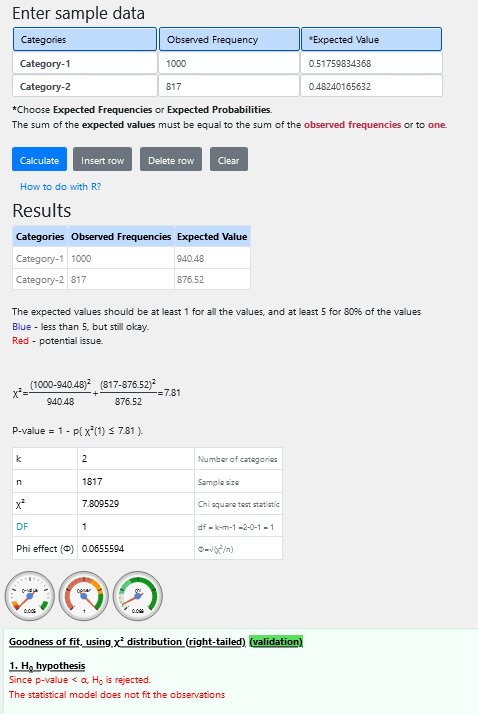
\includegraphics[width=0.75\textwidth]{proof.png}
        \end{center}
    \end{figure}
    \item Please follow the journal guidelines for authors. The figures are not numbered and the legend is not at the end of the document, separated from the figures, as indicated.\\
    \textbf{Minor change}
    \item  In Table 1 you must specify the meaning of the words: "PLEVA", "SLE", "MCTD", "STI", "ADR", "TEN", "HSP", "BCC" and "SCC"\\
    \textbf{Minor change}
    \item  It is worrisome that patients with a "lichen simplex chronicus" and "giant molluscum contagiosum" diagnosis have longer median hospital stays than those of "pemphigus vulgaris". Could you please give an explanation for this?
    \item Could you please explain why for diseases with only one patient (pityriasis rosea, lichen simplex chronicus, DRESS syndrome, kerion, SCC) a median statistic was calculated, how was it obtained? \\
    \textbf{While claculation of central tendency is non standard for samples with single data point, we did it for the sake of completeness. If needed, we can remove it too!}
    \item You mention: “The mean length of admission was 9.6 ± 10.2 (median: 6; range: 1 to 81) days”, what is the reason for obtaining both mean and median?\\
    \textbf{The standard deviation was noted to be quite high, sometimes even greater than the mean. This suggests an inherent skewness in the data, which needed attention in our opinions.}

\section{Discussion and Bib}

Minor changes


\end{enumerate}

\end{document}